\section{背景及相关工作}

\subsection{基于GPU的机器学习应用与CUDA}

\subsubsection{基于GPU的机器学习应用}
\par 随着当今机器学习,尤其是深度学习应用中数据量、网络结构复杂度的增长,该类应用对于硬件计算能力的要求也迅速增长。而在这类应用中,有许多密集的计算互相之间是没有数据/控制依赖的,也就是可以并行执行的;比如神经网络前向、反向传播中的权重矩阵计算,这些权重在同一轮计算中不存在耦合性;随机森林(Random Forest)中不同分类器的训练,这一特征可以利用到GPU处理中流这一特征;一系列聚类算法,包括DBSCAN、K-Means等;而图形处理单元(GPU)的设计初衷正是大规模并行计算,也因为GPU的计算能力,深度学习自上世纪末至今迅猛发展,同时GPU的运算性能以及相应的软件的发展也非常迅速。目前,GPU更多代表了通用处理单元(General Purpose)。
\par 当然,GPU上的编程模型与CPU上的模型有较大差别,为了方便程序员搭建模型,目前市面上的许多框架包括TensorFlow, PyTorch, PyChain等都更新了对GPU的支持。然而,这些框架方便了程序员的程序编写,抽象了底层硬件的细节,比如在CUDA中,线程块、线程束的调度以及相应寄存器文件的分配会对程序性能造成极大影响,然而这些特征都被框架抽象这就导致了硬件性能无法得到完全的发挥。且目前大部分框架都是基于老架构与老SDK编译,没有对新架构与新SDK做出优化。本文的目的也是在于挖掘出新架构的硬件以及对应的新的SDK中的代码翻译、指令执行等部分的特征以及相较老架构和老SDK的变化;根据分析得出的结论修改已有GPU程序的源码,尝试修改某些框架的源码,并给出实际的修改、编程时的建议。
\subsubsection{CUDA}
\par CUDA (Compute Unified Device Architecture)是由英伟达(Nvidia)针对图形处理单元开发的并行计算平台及对应的编程模型。在编写CUDA程序时,程序员通过在一些较为热门的语言包括C/C++、Python、MATLAB、Fortran中以关键字的形式加入扩展来描述并行行为\parencite{CUDAZONE}。下面将介绍CUDA程序的编程模型、编译过程与调用/执行方式。
\paragraph{编程模型}
\par 在介绍编程模型前,需要简要介绍一下Nvidia GPU的硬件结构。自顶向下的结构为:一块GPU芯片有若干流多处理器单元(Stream Multiprocessor,SM),这些流多处理器单元被一个线程块调度器管理,所有流多处理器单元通过全局内存总线和常量内存总线经过L2缓存共享全局内存与常量内存,这部分内存自费米架构以来有GDDR4、GDDR5、GDDR5X、GDDR6X、HBM、HBM2等类型。每个流多处理器单元中有若干个流处理器(Stream Processor,SP),因CUDA程序为SIMT(单指令多线程)并行方式,所以这些流处理器共享一个指令缓存,每个流处理器拥有自己的线程束调度器与寄存器文件;流处理器中包含若干种执行单元,有浮点单元,整数单元,在新架构中还加入了张量单元(Tensor Core),在RTX 2080TI上具体的参数为:一个SM包含64个单精度浮点算术单元,32个双精度浮点算术单元,64个32位整形算术单元,8个混合精度张量单元,4个线程束调度器和16个特殊功能单元;所有流处理器通过显存纵横矩阵(CrossBar)访问共享内存,或被称为L1缓存\parencite{EXPLORING},所有流多处理器共享L2缓存。
\par 因本文的工作主要基于C/C++完成,故只介绍CUDA C/C++的编程模型。在保证相关环境配置完成后,向C/C++源码中加入CUDA相关工具是十分方便的。首先需要确定哪些任务需要在CPU上执行,哪些在目标硬件GPU)上执行;选择的标准一般是考察其数据/控制依赖,依赖性小、计算密集的可以考虑在GPU上执行。确定完毕后编写CPU端和GPU端的函数,有如图\ref{Fig.1}中所示的三种函数。
\begin{figure}
	\centering
	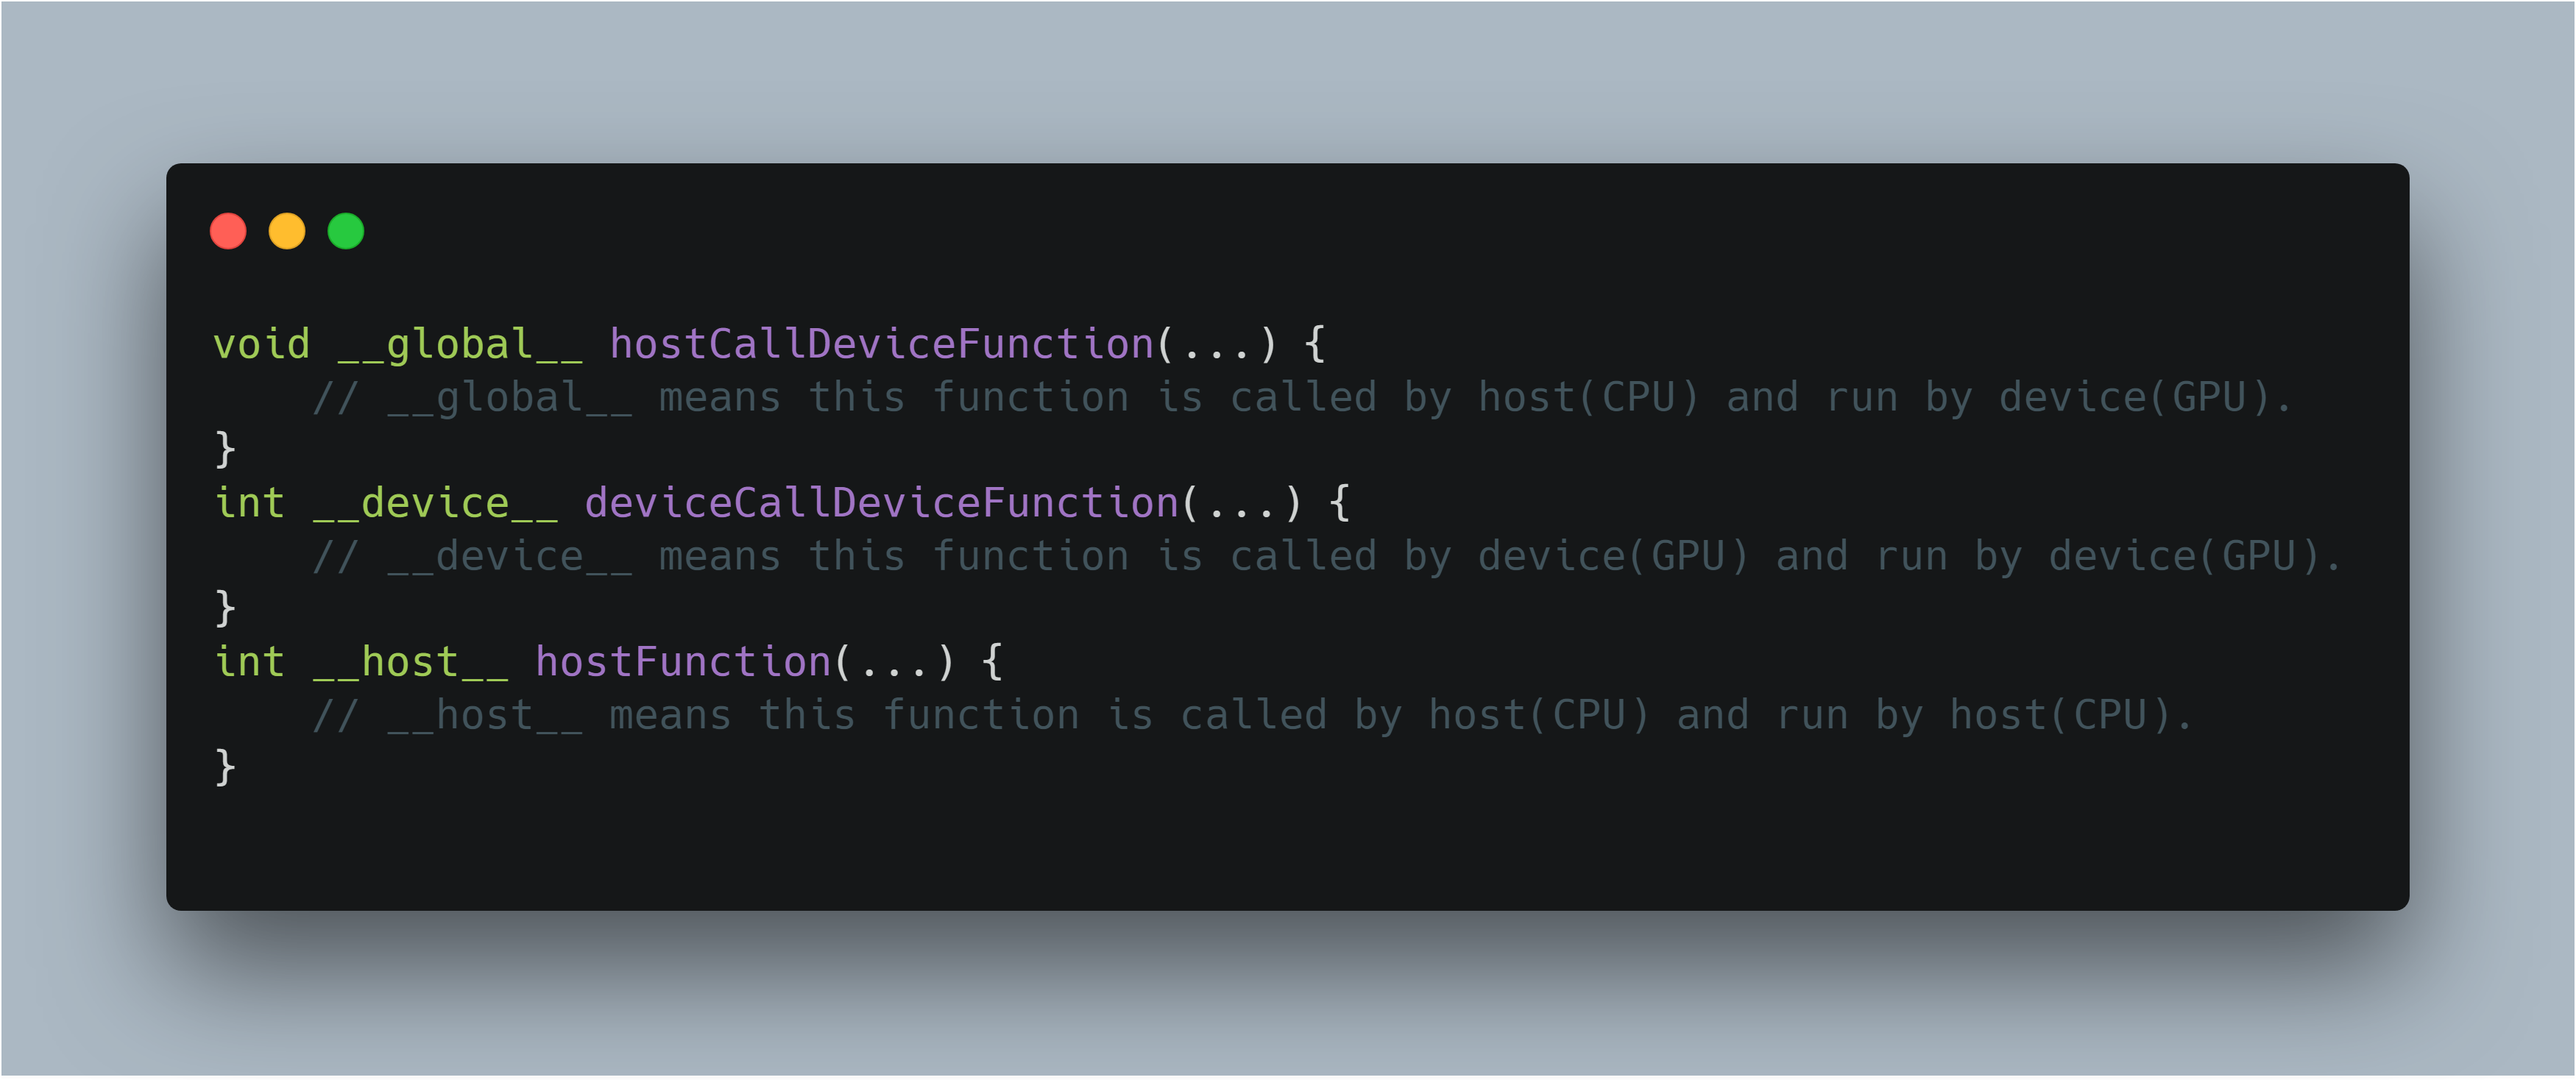
\includegraphics[width=15cm]{figures/CODE1.png}
	\caption{\label{Fig.2} CUDA中的三种函数}
\end{figure}
\par 以上代码段加粗部分为CUDA关键字,对于函数有三种修饰:\_\_global\_\_, \_\_device\_\_, \_\_host\_\_. 分别代表被CPU调用运行于GPU、被GPU调用运行于GPU和被CPU调用运行于CPU的函数。其中被CPU调用运行于GPU的函数只能拥有void返回值,且所有运行于GPU的函数都不支持可变参数列表\parencite{EVENEASIER}。\_\_device\_\_和\_\_host\_\_关键字修饰的函数的调用方式与传统函数别无二致,\_\_global\_\_关键字修饰的函数调用方式如图\ref{Fig.4}所示。
\begin{figure}
	\centering
	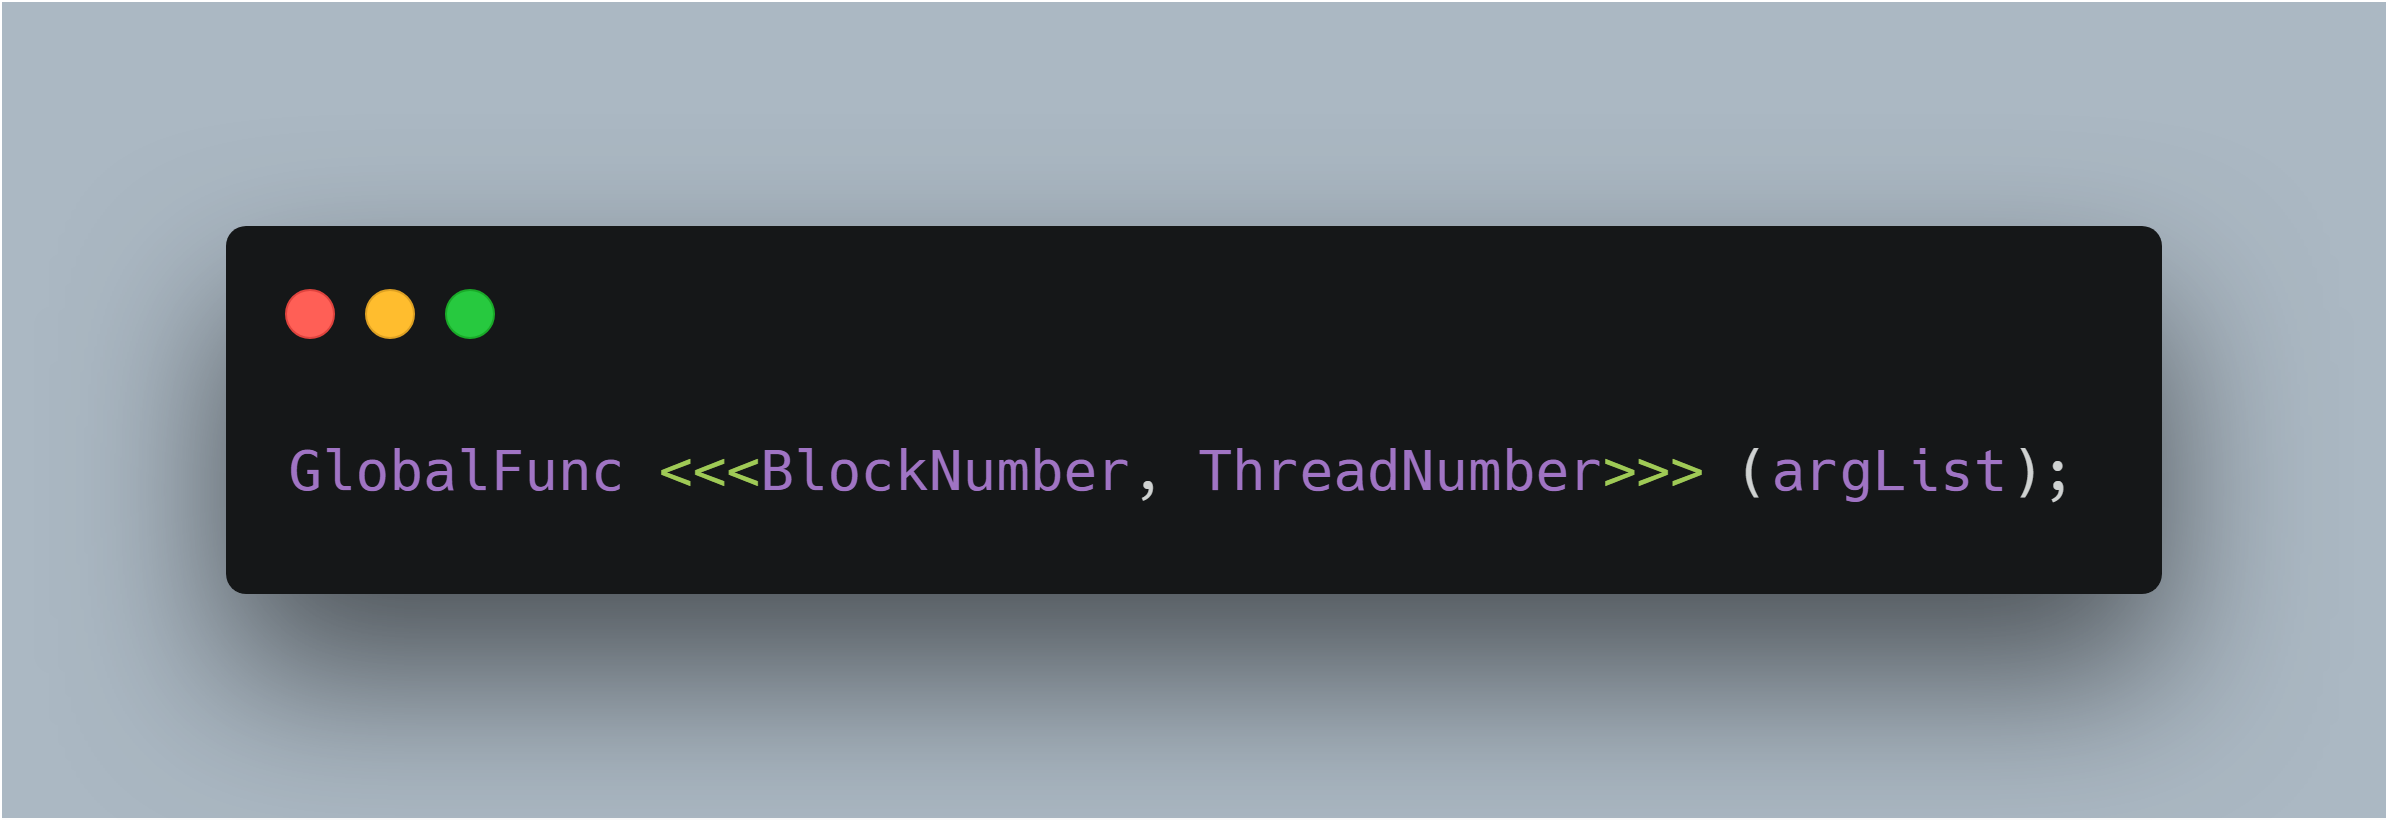
\includegraphics[width=15cm]{figures/CODE3.png}
	\caption{\label{Fig.4} \_\_global\_\_函数调用方式}
\end{figure}
BlockNumber和ThreadNumber分别代表要启动的线程块数目和每个线程块中线程的数目,这一部分取值对程序性能影响较大,之后会详细说明。

\par 之前提到了GPU端的缓存,CUDA程序的另一个重点是存储系统的管理。传统CPU编程模型中,寄存器、缓存等资源都是由CPU自行管理,而不开放给程序员。其原因在于CPU拥有的寄存器、缓存资源较为紧缺,为提高指令级并行能力,需要采用多队列乱序发射与寄存器重命名等技术。相对得,GPU有较为充足的物理寄存器、缓存资源,程序员也对这部分资源掌握有一定的控制权\parencite{CUDAPROG}。CUDA中的存储设备如表所示。
\begin{center}
	\begin{tabular}{cccc}
		\toprule
		项目				&	大小			&	延迟(时钟周期)	&	访问权限	\\
		\midrule
		寄存器文件		&	8KB-64KB/SM		&	$ 10^0 $	& GPU端	\\
		共享内存(L1,L2)	&	16KB-128KB/SM	&	$ 10^1 $	&	GPU端\\
		常量内存		&	N/A				&	N/A		&	N/A	\\
		纹理内存		&	N/A				&	N/A		&	N/A \\
		全局内存		&	-GB				&	$ 10^2 $	&	CPU端/GPU端 \\
		\bottomrule
	\end{tabular}
\end{center}
\par 需要注意的是,常量内存与纹理内存都是全局内存的一种虚拟地址形式。和常量内存一样,纹理内存也是一种只读内存;但是在缓存加载的行为方面,常量内存与传统方式一样,加载所访问数据单元的所在行的一部分单元,而纹理内存则加载所访问数据周围一个范围内的单元\parencite{THEDESIGN}。这样做的原因是在GPU进行图形运算时,处理某一像素点需要用到周围一个范围内所有像素点的信息比如进行抗锯齿作业时,而非只有一行,如图\ref{Fig.1}所示。采用这种结构能改善某些访问模式情况下程序的性能。
\par 这些内存的使用方式如图\ref{Fig.3}所示。寄存器和共享内存的使用方式很好理解,关于常量内存和纹理内存,由于他们是全局内存中的虚拟地址,故声明常量内存的语句也就是用了全局内存;纹理内存的使用则需要借助相应API。而一般的全局内存的读写权限同时开放给CPU和GPU,故需要使用特定的API进行访问。
\begin{figure}
	\centering
	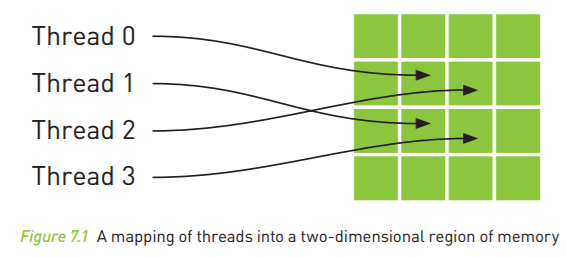
\includegraphics[width=15cm]{figures/Fig1.jpg}
	\caption{\label{Fig.1} 纹理内存访存方式}
\end{figure}
\begin{figure}
	\centering
	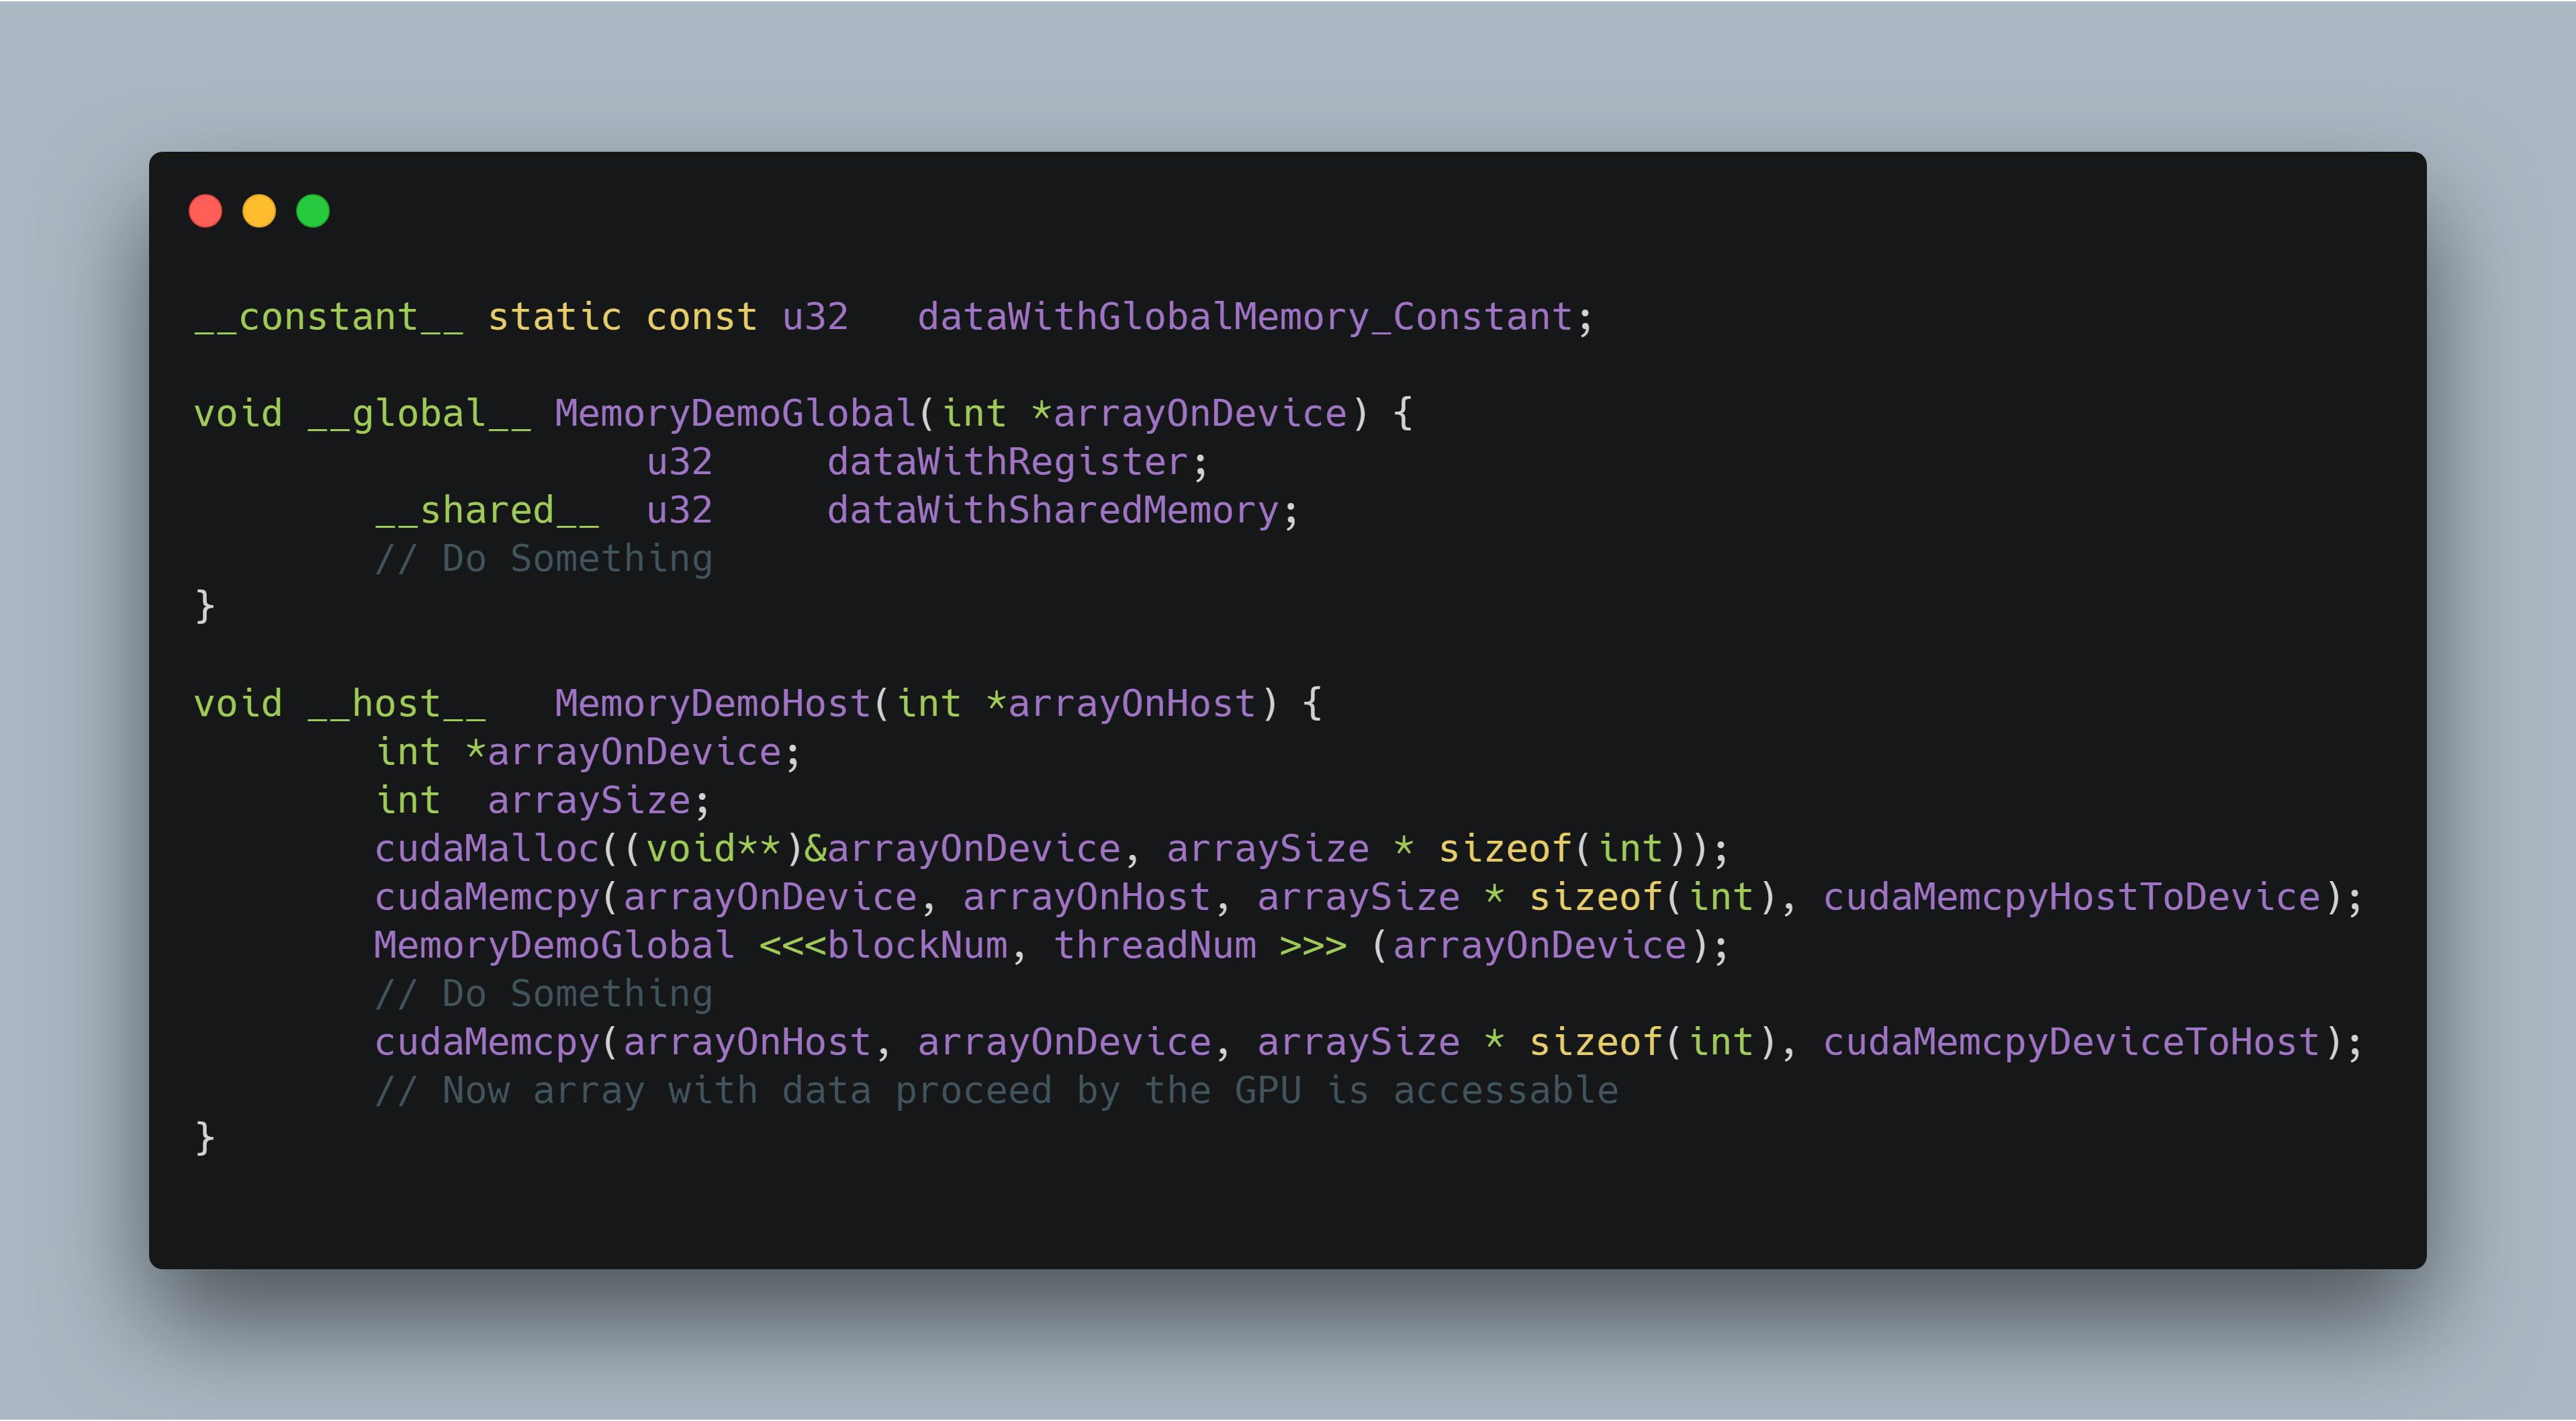
\includegraphics[width=15cm]{figures/CODE2.png}
	\caption{\label{Fig.3} 不同存储系统使用方式}
\end{figure}
\paragraph{编译方式}
\par CUDA程序的编译较为简单,只需使用$ nvcc $对源文件进行编译生成可执行文件。首先将从C/C++/CUDA文件编译生成PTX中间代码,再从PTX中间代码生成SASS机器代码。本实验中由于需要观察、研究具体GPU代码的生成方式、特征,故在编译时加入$ --keep $保留编译产生的PTX中间代码文件。而SASS机器代码则在NVIDIA的支持下通过捕捉CUDA应用的指令流获得。
\paragraph{运行模式}
\par 关于如何从CPU端(host)启动GPU端(device)的函数将在下一节通过CPU端应用程序的反汇编代码详细描述,这一节仅介绍GPU相关的部分。
\par 根据弗林分类法\parencite{FLYNN},计算机系统可以分为SIMD, MIMD, SISD, MISD等类型,目前多核心CPU系统就是MIMD系统。而NVIDIA的GPU系统被称为SIMT(单指令多线程),与SIMD(单指令多数据)有所不同。在这种模型中,一条指令并非仅仅代表一个固定的功能,而是代表执行这一指令的类型、使用的管道/流水线。线程需要执行的具体操作需要编写相关内核代码。直观的特征便是再PTX中间代码和SASS机器代码中,所有的逻辑操作指令都是$ lop/lop3 $,通过后缀$ .and/.or, .sync/.async $指明具体运算和调度特征。所以,在SIMT模型中,内核程序读入统一的数据,程序代码根据需要进行不同操作;实际调度时不同操作通过重复指令流按顺序发射,只不过运算单元会屏蔽无关线程。
\par 首先需要介绍一下计算能力,此处计算能力指的是GPU中流多处理器(SM)支持的运算的等级,分为Major和Minor等级,可以等价为流多处理器的代号,所支持的运算不同。其中Major代号代表架构的更新,这也会带来许多新的硬件支持的运算,而Minor代号则代表同一架构下不同定位的流多处理器产品。如伏特架构的计算能力为7.2,图灵架构的计算能力为7.5,Major代号一样就代表这两种架构其实并无太大修改,而Minor代号则代表伏特架构中流多处理器的类型是Heavy,图灵架构中流多处理器的类型是Lite。Lite和Heavy一般用于区分消费级/工作站级GPU,分别对应GeForce和Tesla代号。
\par 基于GPU的应用与传统的基于CPU的应用在运行方式上有较大差别,主要有以下几点。
\begin{itemize}
	\item GPU中由大量的物理寄存器,达几十~几百KB,且都能在1个时钟周期内访问,而CPU中物理寄存器资源极为有限。故在进行上下文切换时,GPU只需更改寄存器文件指针来切换,而CPU需要使用堆栈保存上下文。
	\item CPU仅仅支持数十个硬件线程,而GPU则支持数千个硬件线程。在GPU上开启过少的硬件线程会极大降低硬件使用率,进而导致性能降低。具体开启线程数量取决于硬件SM最大并发线程数、最大并发线程束数和最大并发块数等。表\ref{table-占用率}显示了在不同计算能力上开启不同数量的线程时设备的利用率以及所能开启包含该数量线程的线程块的数量。\\
	\begin{center}
	\begin{tabular}{cccccc}
		\toprule
			&	1.0	&1.2	&2.0	&2.1	&3.0 \\
		\midrule
		64	&	67\%, 8		&	50\%, 8		&	33\%, 8		&	33\%, 8		&	50\%, 16	\\
		96	&	100\%, 8	&	75\%, 8		&	50\%, 8		&	50\%, 8		&	75\%, 12	\\
		128	&	100\%, 6	&	100\%, 8	&	67\%, 8		&	67\%, 8		&	100\%, 10	\\
		256	&	100\%, 3	&	100\%, 4	&	100\%, 6	&	100\%, 6	&	100\%, 8	\\
		512	&	67\%, 1		&	100\%, 2	&	100\%, 2	&	100\%, 3	&	100\%, 4	\\
		1024&	N/A, N/A	&	N/A, 1		&	67\%, 1		&	67\%, 1		&	100\%, 2	\\
		
		\bottomrule
	\end{tabular} \label{table-占用率}
	\end{center}
	可见,随着计算能力的增长,一个流多处理器上所能容纳的线程束月俩月多。在充分利用寄存器文件和共享内存(L1缓存)的情况下开启线程数越多,设备利用率越高。然而过多的线程会导致资源紧缺,在实际使用中应当根据硬件参数,问题规模做出调整。
\end{itemize}
\par 在CUDA程序中,32个线程被组织成一个线程束(warp),作为基本的调度单元,具有各自的物理寄存器,也就是说线程束中32个线程一般情况下都会执行相同指令流,为SIMD模式。在目前的图灵架构中,线程束仍然是同步的单位,即线程束之间可以保证同步,线程束内部线程无法保证同步。在下一代安培架构(Ampere)则引入$ Arrive-Wait $模式以实现线程级别同步,以提高CUDA程序的灵活性。 
\par 若干个线程束被组织为一个线程块(block),在下一代安培架构中将添加一个线程束组的层级(warp group),由四个线程束组成,但该层级仅为大规模通用矩阵乘法运算所用(Ultra MMA),且本代架构还未应用,这里不做讨论。线程块中的线程束可以通过\_\_syncthread()进行同步,线程块中的线程能够访问共享内存进行数据交换。一个线程块被分配在一个流多处理器上执行,一个流多处理器能分配多个线程块。
\par 若干个线程块被组织成一个线程网格(grid),线程网格可被看作一个分配给GPU的任务。
\par 表\ref{table-粒度}详细说明了CUDA应用中不同不同粒度的线程组织形式。
\begin{center}
	\begin{tabular}{ccc}
		\toprule
		粒度	&	调度者	& 	分配给 \\
		\midrule
		warp		&	流多处理器内部调度器	&	流处理器(Stream Processor)\\
		block(CTA)	&	TPC调度器(MPC)		  &		流多处理器(Stream Multi-processor)\\
		grid		&	GPC调度器(GPM)		  &		TPC(Texture Processing Cluster)$ * $\\
		kernel		&	CPU, PCIe			&		GPC(Graphics Processing Cluster)	\\	
		\bottomrule
	\end{tabular} \label{table-粒度}\\

$ * $ 在本世代图灵架构及以前,TPC与SM可以等价,因为一个TPC上仅包含一个SM,然而自下一代安培架构开始,一个TPC中将会有若干个SM。虽然本文研究的图灵架构的硬件在逻辑上SM与TPC等价,但在硬件上还是会做区分,故在表中详细写出。
\end{center}
\subsection{目前展开的工作}

\subsection{CUDA应用的汇编代码与PTX中间代码的结构}

\subsubsection{CUDA应用汇编代码结构}

\subsubsection{PTX中间代码结构}